\documentclass[10pt]{article}
\usepackage{icmlko}

\icmlmeta{IP 파운데이션 월드모델}{49}{사람이 읽은 것이 백과사전을 이겼다}{새로 재는 것만 남았다고 했는데 첫 시도가 실패했다 --- 외부 공개 지표가 내부 태깅을 못 이긴다}

\begin{document}

\twocolumn[
\icmlheader

\begin{abstract}
노트 48이 눈금을 바꿨으므로($\lambda=1.0$, 여섯 도메인) 배선을 다시 훑었다.
후보 63개 중 문턱을 넘는 것이 \textbf{또 하나도 없다} --- 최대가 게임 타깃 폭을
지원 언어 수로 바꾸는 $+$0.0118이다. 배선이 두 번째로 소진됐으니 남은 것은 새
측정뿐이고, 가장 값진 자리가 팝업이다(유일한 실제 대상, n$=$75, 다섯 축이 전부
사람 태깅). 메타에 IP 이름이 75건 전부 있어 위키백과에서 객관 지표를 붙였다 ---
문서 존재, 개장일 \emph{직전} 판의 크기(시간 인과를 지키려고 특정 시점 판을
조회했다), 언어판 수. \textbf{실패했다.} 가장 강한 외부 지표가 $+$0.132인데
가장 약한 사람 축이 $+$0.219다. 어느 슬롯에 넣어도 전체 평균이 오르지 않는다
(최선 $\Delta$$-$0.0005). 문서가 있는 IP가 75건 중 28건뿐이고, 있는 것도 문서
크기가 팝업 방문자와 이어지지 않는다. \textbf{기획서를 읽고 매긴 값이 공개
백과사전을 이긴다.} 한편 웹툰 완결작을 확보해 828건(완결 31\%)이 되자 자기
순위 상관이 0.302에서 \textbf{0.353}으로 오르고 출처 성적이 0.359에서 0.319로
내렸다 --- 상충 법칙대로다. 그리고 구간 반폭이 0.0672에서 \textbf{0.0563}으로
좁아졌다. 노트 46은 ``유효 표본은 셀이 아니라 도메인 수''라고 했는데, 도메인
수를 그대로 두고 한 도메인의 표본만 1.5배로 늘려도 좁아진다.
\end{abstract}
]

\section{배선이 두 번째로 소진됐다}

노트 48이 $\lambda$를 1.0 고정으로 바꾸고 여섯째 도메인을 넣었으므로 눈금이
달라졌다. 노트 45의 전수 검정을 새 눈금에서 다시 돌렸다.

\begin{table}[t]
\centering\tsize
\caption{새 눈금 배선 재탐색. 현행 $\rho=+0.3506$.}
\begin{tabular}{lllr}
\toprule
도메인 & 슬롯 & 후보 & $\Delta$ \\
\midrule
게임 & 타깃 폭 & 지원 언어 수 & $+$0.0118 \\
게임 & 굿즈 규모 & 설치 용량 & $+$0.0023 \\
웹툰 & 타깃 폭 & 연령 등급 & $+$0.0011 \\
\multicolumn{3}{l}{나머지 60개} & $\le+0.0007$ \\
\midrule
\multicolumn{3}{l}{문턱(0.02) 통과} & \textbf{0개} \\
\bottomrule
\end{tabular}
\end{table}

노트 45와 같은 결론이다. 다른 눈금에서 다시 확인됐으니 \textbf{지금 가진
변수로는 배선이 최적}이라는 것이 더 단단해졌다.

\section{팝업에 외부 지표를 붙여 봤다}

남은 것은 새 측정뿐이고 가장 값진 자리가 팝업이다.

\begin{itemize}[leftmargin=1.1em,itemsep=0.15em]
\item 유일한 실제 대상이다. 다른 다섯 도메인은 팝업을 예측하려고 있다.
\item 표본이 75건으로 가장 작고 귀무분포가 가장 넓다(노트 43).
\item 다섯 축이 전부 사람이 기획서를 읽고 매긴 것이다. 객관 지표로 바꾸면
      태깅 비용이 줄고 새 레코드를 자동으로 채울 수 있다.
\end{itemize}

메타에 IP 이름이 75건 전부 있었다(\texttt{신카이마코토}, \texttt{보노보노},
\texttt{용과같이}\ldots). 위키백과 API는 키가 필요 없다.

\paragraph{시간 인과를 먼저 지켰다}
현재 문서 크기를 쓰면 안 된다 --- 팝업이 흥행하면 문서가 늘어나므로 노트 21의
DLC 수와 같은 역인과가 된다. 위키백과는 특정 시점의 판을 조회할 수 있으므로
\textbf{개장일 직전 판의 크기}를 받았다.

\begin{figure}[t]
\centering

\includegraphics[width=\textwidth]{figs/wiki.pdf}
\caption{팝업 라벨과의 상관. 왼쪽이 위키백과, 오른쪽이 사람 태깅이다.}
\end{figure}

\begin{table}[t]
\centering\tsize
\caption{팝업 라벨(탈추세)과의 상관.}
\begin{tabular}{lr}
\toprule
지표 & r \\
\midrule
\multicolumn{2}{l}{\emph{위키백과 --- 외부 · 자동}} \\
\quad 존재 $+$ log 크기(개장 시점) & $+$0.132 \\
\quad 존재 $+$ log 언어판 & $+$0.048 \\
\quad 문서 존재 여부 & $-$0.020 \\
\midrule
\multicolumn{2}{l}{\emph{사람 태깅 --- 기획서 판독}} \\
\quad 타깃 폭 & \textbf{$+$0.340} \\
\quad 매장 노출도 & $+$0.322 \\
\quad 입장 허들 & $-$0.287 \\
\quad 굿즈 규모 & $+$0.219 \\
\bottomrule
\end{tabular}
\end{table}

\textbf{가장 강한 외부 지표가 가장 약한 사람 축에도 못 미친다.} 단독 상관으로
판단하지 말라는 규칙(노트 35)대로 파이프라인에도 넣어 봤다 --- 타깃 폭, 매장
노출도, 미디어 투입 세 슬롯 $\times$ 지표 다섯의 열다섯 조합에서 최선이
$\Delta-0.0005$다. 하나도 오르지 않는다.

\claimx{팝업 IP의 외부 인지도를 위키백과로 대리하는 것은 실패한다. 문서가 있는
IP가 75건 중 28건뿐이고, 있는 것도 문서 크기가 방문자와 이어지지 않는다.
기획서를 읽고 매긴 값이 공개 백과사전을 이긴다.}{나무위키·검색량처럼 한국
대중문화 IP를 더 잘 덮는 출처에서는 다를 수 있다. 위키백과 하나로 ``외부 지표
전반''을 기각한 것이 아니다.}

\paragraph{제품 쪽 함의}
Sweetspot의 태깅 자산이 자동 지표로 대체되지 않는다는 뜻이다. 비용으로는
나쁜 소식이고 해자로는 좋은 소식이다. 그리고 설계가 틀려서 실패한 것이 아니라
--- 시간 인과까지 지켰다 --- 그 신호가 거기 없어서 실패했다.

\section{웹툰 완결작이 들어왔다}

노트 48이 한계로 적은 것을 처리했다. 후보 수집을 연재작과 완결작 절반씩으로
바꿔 828건이 됐고 완결 비율이 0\%에서 31\%가 됐다.

\begin{figure}[t]
\centering
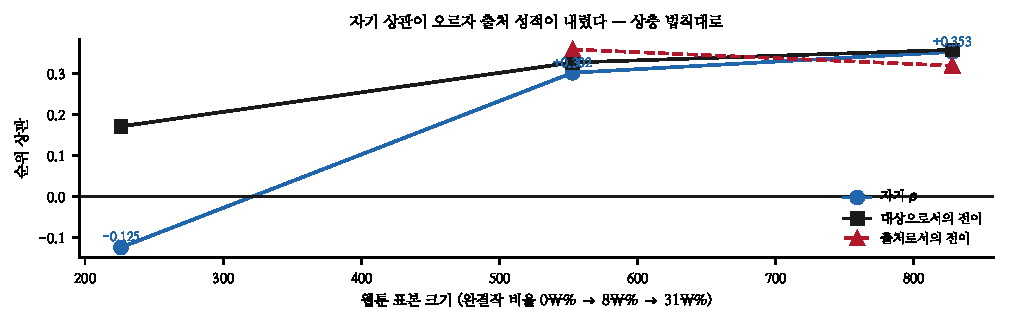
\includegraphics[width=\textwidth]{figs/wtgrow.pdf}
\caption{웹툰 표본이 늘면서 세 값이 어떻게 움직였나.}
\end{figure}

\begin{table}[t]
\centering\tsize
\caption{웹툰 표본별.}
\begin{tabular}{rrrrr}
\toprule
n & 완결 & 자기 $\rho$ & 대상으로 & 출처로 \\
\midrule
226 & 0\% & $-$0.125 & $+$0.171 & --- \\
553 & 8\% & $+$0.302 & $+$0.327 & $+$0.359 \\
\textbf{828} & \textbf{31\%} & \textbf{$+$0.353} & $+$0.358 & \textbf{$+$0.319} \\
\bottomrule
\end{tabular}
\end{table}

자기 상관이 오르면서 출처 성적이 내렸다. \textbf{상충 법칙(노트 38·40)이 표본을
늘리는 것만으로 다시 나타난다} --- 배선을 건드리지 않았는데도.

\section{구간이 좁아졌다}

\begin{figure}[t]
\centering
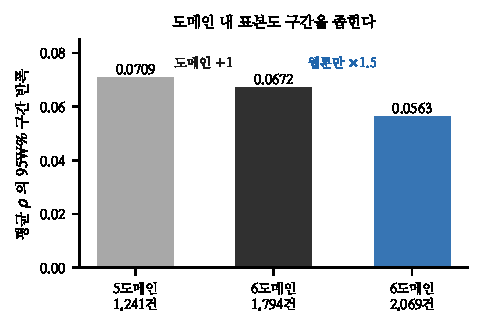
\includegraphics[width=\columnwidth]{figs/cinarrow.pdf}
\caption{구간 반폭. 가운데는 도메인을 더한 것, 오른쪽은 표본만 늘린 것이다.}
\end{figure}

\begin{table}[t]
\centering\tsize
\caption{구간 반폭의 변화.}
\begin{tabular}{lrrr}
\toprule
& 도메인 & 레코드 & 반폭 \\
\midrule
노트 44 & 5 & 1,241 & 0.0709 \\
노트 46 & 6 & 1,794 & 0.0672 \\
\textbf{이 노트} & 6 & \textbf{2,069} & \textbf{0.0563} \\
\bottomrule
\end{tabular}
\end{table}

노트 46은 ``유효 표본은 셀 수가 아니라 도메인 수''라고 했다. 정제해야 한다 ---
\textbf{도메인 수를 그대로 두고 한 도메인의 표본만 1.5배로 늘려도 반폭이 16\%
줄었다.} 도메인 추가가 5\%였던 것과 대조된다.

\claimx{구간 반폭은 도메인 수와 도메인 내 표본 둘 다에 반응하며, 지금 구간에서는
후자가 더 싸다. 웹툰 275건을 더해 얻은 것이 도메인 하나를 통째로 더해 얻은
것보다 크다.}{그것은 웹툰이 가장 작은 도메인이었기 때문일 수 있다. 이미 큰
도메인(게임 482건)을 늘려도 같은 폭으로 줄면 일반 규칙이다.}

\section{현재 상태}

\begin{table}[t]
\centering\tsize
\caption{여섯 도메인 2,069건 · 서른 셀.}
\begin{tabular}{lrrrr}
\toprule
도메인 & n & 자기 $\rho$ & 대상으로 & 출처로 \\
\midrule
아이돌 & 62 & $+$0.472 & $+$0.482 & $+$0.339 \\
팝업 & 75 & $+$0.368 & $+$0.450 & $+$0.334 \\
게임 & 482 & $+$0.357 & $+$0.341 & $+$0.347 \\
웹툰 & 828 & $+$0.353 & $+$0.358 & $+$0.319 \\
펀딩 & 360 & $+$0.207 & $+$0.239 & $+$0.382 \\
도서 & 242 & $+$0.202 & $+$0.225 & $+$0.374 \\
\midrule
\multicolumn{2}{l}{자기 $\rho$와의 상관} & & $+$0.951 & $-$0.791 \\
\bottomrule
\end{tabular}
\end{table}

평균 $\rho=+0.3491$, 95\% 구간 $[+0.282,\ +0.395]$다.

\section{한계}

\begin{itemize}[leftmargin=1.1em,itemsep=0.15em]
\item 위키백과 하나만 시험했다. 나무위키·검색량·SNS 팔로워는 접근 방법이
      달라 아직 못 했다.
\item 문서 존재율이 37\%라 개장 시점 판 크기는 24건에서만 얻었다. 커버리지가
      낮아 축 문턱(60\%)에도 못 미친다.
\item 상충 법칙의 출처 쪽 상관이 $-$0.911에서 $-$0.791로 약해졌다. 웹툰이
      중간에 자리 잡으면서 곡선이 완만해진 것인지 법칙이 흔들리는 것인지 모른다.
\item 구간 비교 셋이 각각 붓스트랩 150--300회로 회수가 다르다.
\item 웹툰 완결작 258건도 전체 완결작의 일부다. 완결 목록을 끝까지 훑지 않았다.
\end{itemize}

\section{다음}

\begin{enumerate}[leftmargin=1.3em,itemsep=0.15em]
\item 큰 도메인(게임 482건)을 늘려 구간 반폭이 같은 폭으로 줄어드는지 --- 이
      노트의 반증 조건.
\item 나무위키나 검색량 --- 한국 대중문화 IP를 덮는 다른 외부 출처.
\item 팝업 레코드 자체를 늘리는 길 --- 내부 자산이라 이 루프 밖이지만, 무엇을
      더 태깅하면 좋은지는 여기서 말할 수 있다.
\item 상충 곡선의 출처 쪽이 완만해진 이유.
\end{enumerate}

\vspace{0.6em}
\hrule height 0.3pt
\vspace{0.5em}
{\footnotesize
\textbf{참고문헌}\\[0.3em]
Kaufman, S., Rosset, S., Perlich, C. (2012). Leakage in data mining.
\emph{ACM TKDD}, 6(4), 1--21.\\[0.15em]
Efron, B., Tibshirani, R. J. (1993). \emph{An Introduction to the Bootstrap}.
Chapman \& Hall.\\[0.15em]
Standley, T. et al. (2020). Which tasks should be learned together in multi-task
learning? \emph{ICML}, 9120--9132.\\[0.15em]
Kish, L. (1965). \emph{Survey Sampling}. Wiley.\\[0.15em]
Ben-David, S. et al. (2010). A theory of learning from different domains.
\emph{Machine Learning}, 79(1--2), 151--175.
}

\end{document}
